\documentclass[margin=5mm]{standalone}
\usepackage[dvipsnames]{xcolor}
\usepackage{pgfplots}
\usepackage{tikz}

\pgfplotsset{compat=1.18}
\begin{document}

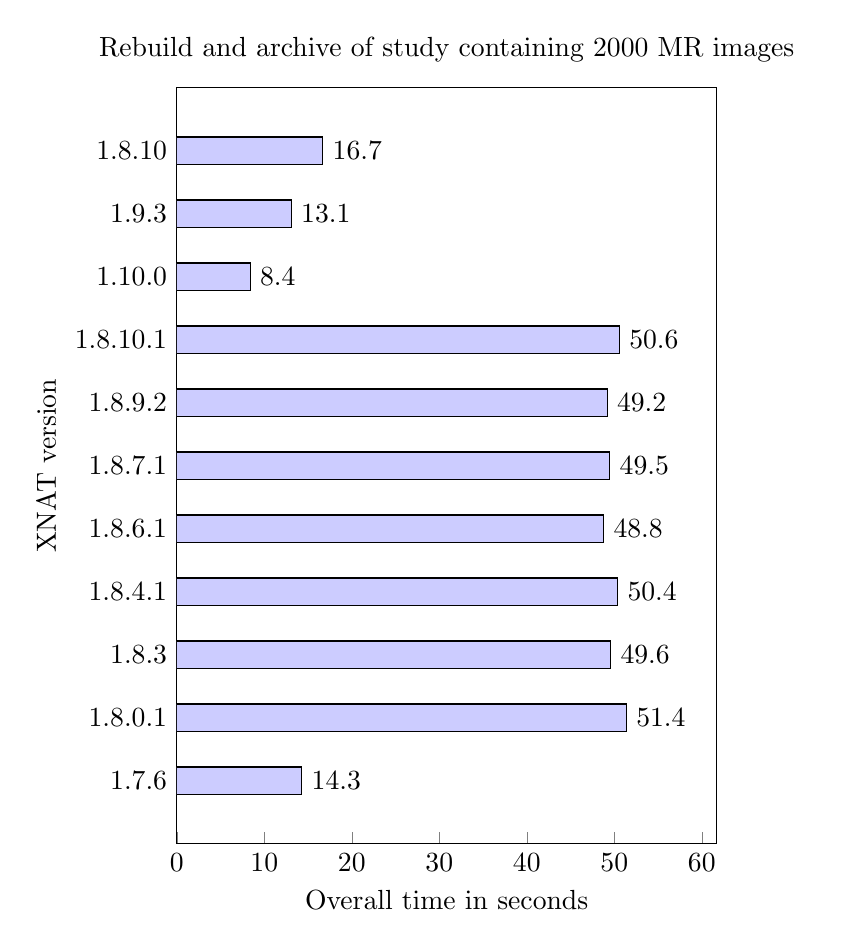
\begin{tikzpicture}
    \begin{axis}[
        align = center,
        xlabel = Overall time in seconds,
        ylabel = XNAT version,
        xtick pos = left,
        ytick pos = left,
        ytick = data,
        xmin = 0,
        enlarge x limits = {value = 0.2, upper}, % make node labels not overlap with axes
        title = {Rebuild and archive of study containing 2000 MR images},
        title style = {text width = 0.8\textwidth},
        nodes near coords,
        nodes near coords align = horizontal,
        symbolic y coords = {1.7.6,1.8.0.1,1.8.3,1.8.4.1,1.8.6.1,1.8.7.1,1.8.9.2,1.8.10.1,1.10.0,1.9.3,1.8.10},
        enlarge y limits = 0.1,
        y = 0.8cm,
        point meta=x
    ]
        \addplot[xbar, fill = blue!20!white] coordinates { (14.3,1.7.6) (51.4,1.8.0.1) (49.6,1.8.3) (50.4,1.8.4.1) (48.8,1.8.6.1) (49.5,1.8.7.1) (49.2,1.8.9.2) (50.6,1.8.10.1) (8.4,1.10.0) (13.1,1.9.3) (16.7,1.8.10) };
    \end{axis}
\end{tikzpicture}

\end{document}